\documentclass[../../main.tex]{subfiles}

\begin{document}
A continuación, describimos las diferentes arquitecturas de redes neuronales que
utilizamos durante los experimentos y los valores particulares que fueron incluidos en la
búsqueda de hiperparámetros.

Un aspecto a notar sobre nuestros datos es que contienen características temporales (la
serie de tiempo) y ``estáticas'' (el inicio de programa). Lo que hicimos en todas las
arquitecturas fue procesar la serie temporal por un lado y para hacer la clasificación,
combinar el resultado de este procesamiento con la entrada estática.

La salida de cada modelo es un número real que representa la probabilidad que la entrada
dada\footnotemark - caracterizada por la serie de tiempo y el inicio de programa -
pertenezca a la categoría con etiqueta 1, que en nuestro caso representa formar parte del
grupo de control. Para obtener la clase final (0 o 1), se aplica - por fuera del modelo
propiamente dicho - un \textbf{umbral de decisión} sobre esta probabilidad: si la
probabilidad es mayor que dicho umbral, se considera que el modelo ha clasificado a la
entrada como pertenceciente a la clase 1. En este trabajo, fijamos este umbral en 0.5.
\footnotetext{En realidad, lo que producen las redes como salida es un valor real, y no
una proabilidad. Para interpretar este valor como una probabilidad, se debe aplicar una
función sigmoide. PyTorch provee una función de pérdida llamada \texttt{BCEWithLogitsLoss}
que realiza internamente esta ``conversión'' y la inclusión explícita de la función
sigmoide en la arquitectura de la red.}

Dejamos algunos hiperparámetros fijos en todas los modelos:
\begin{itemize}[itemsep=0cm, topsep=0cm, parsep=0cm, partopsep=0cm]
    \item Número de épocas de entrenamiento: 100.
    \item Número de capas para el procesamiento de series temporales: 2.
    \item Optimizador: Adam.
\end{itemize}

Y aquellos sobre los que llevamos a cabo una búsqueda fueron los siguientes:
\begin{itemize}[itemsep=0cm, topsep=0cm, parsep=0cm, partopsep=0cm]
    \item Tamaño de lote: probamos con 32, 64 y 128.
    \item Número de neuronas por capa: probamos 32, 64 y 128.
    \item Tasa de aprendizaje: probamos con 0.01, 0.001 y 0.0001.
\end{itemize}

Para hacer esta búsqueda, utilizamos la técnica de validación cruzada sobre los conjuntos
de entrenamiento, con 3 particiones. La métrica que se buscó optimizar fue el puntaje
\(F_1\) - discutido posteriormente en la sección \ref{sec:metricas} - promediado sobre las
tres iteraciones de la validación cruzada.

En lo que sigue, incluimos ilustraciones y detallamos en profundidad las arquitecturas
utilizadas.

\subsection{Arquitectura 1: Red LSTM}
Como se puede ver en la Figura \ref{fig:lstm_v2}, la primera arquitectura propuesta se
compone, por un lado, de dos capas LSTM con una capa intermedia de dropout, encargadas de
procesar la serie de tiempo. Posteriormente, se realiza una operación de concatenación, en
la que se combina la salida de la ``parte'' LSTM con la característica correspondiente al
inicio del programa en un vector unidimensional que puede ser ``alimentado'' a capas
totalmente conectadas. De esta forma, el vector se introduce en una red densa compuesta
por una capa oculta de 128 neuronas con función de activación ReLU, seguida de una capa de
dropout, y finaliza en una capa de salida que produce la probabilidad final.
\begin{figure}[h]
    \centering
    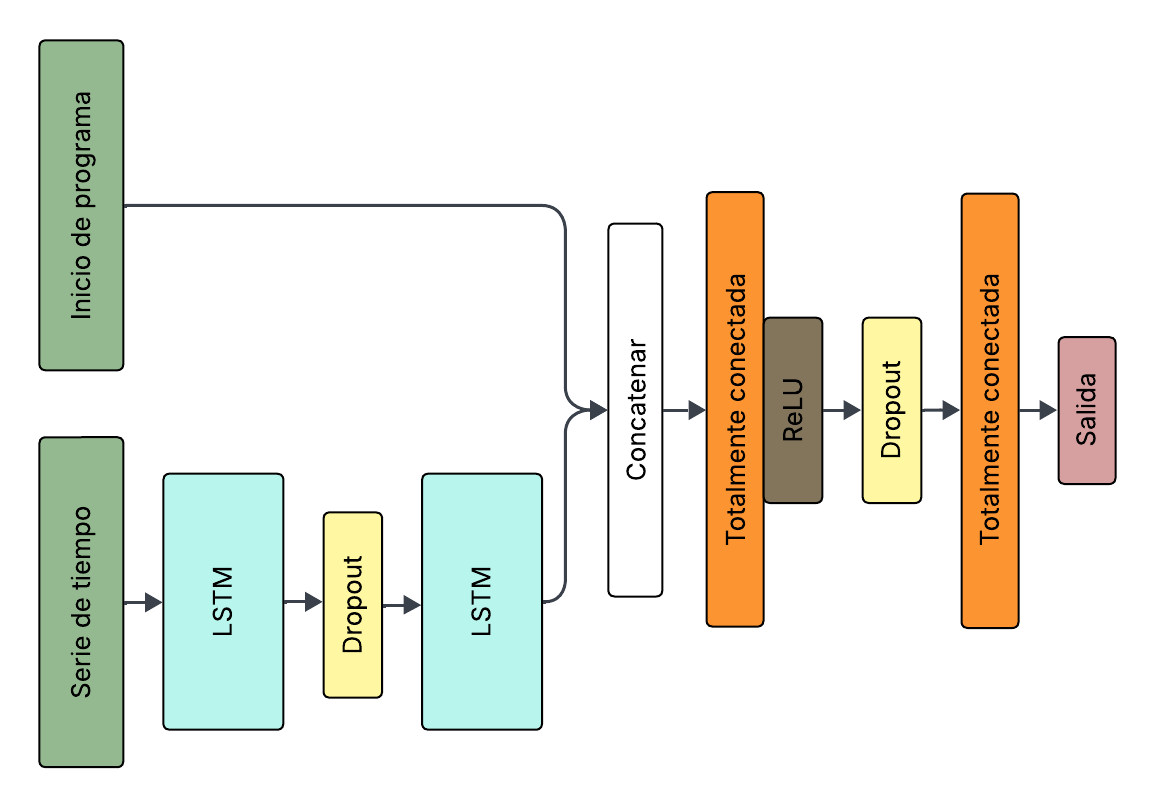
\includegraphics[width=0.7\textwidth]{figs/lstm_v2.png}
    \caption{Esquema de la arquitectura de la red LSTM propuesta.}
    \label{fig:lstm_v2}
\end{figure}

\subsection{Arquitectura 2: Red Convolucional}
El segundo modelo propuesto sigue la misma estructura general que la arquitectura
anterior, pero reemplazando las capas LSTM por capas convolucionales. Concretamente, ahora
el procesamiento de la serie temporal se realiza mediante dos capas convolucionales, cada
una con normalización de lote y ReLU, y entre medio de ellas una capa de dropout. A
continuación, se aplica una segunda capa de \textit{dropout} y una operación de
\textit{average pooling}. Finalmente, la salida resultante se convierte en un vector
unidimensional que alimenta las capas posteriores del modelo. La Figura \ref{fig:conv}
muestra un diagrama de esta arquitectura.
\begin{figure}[h]
    \centering
    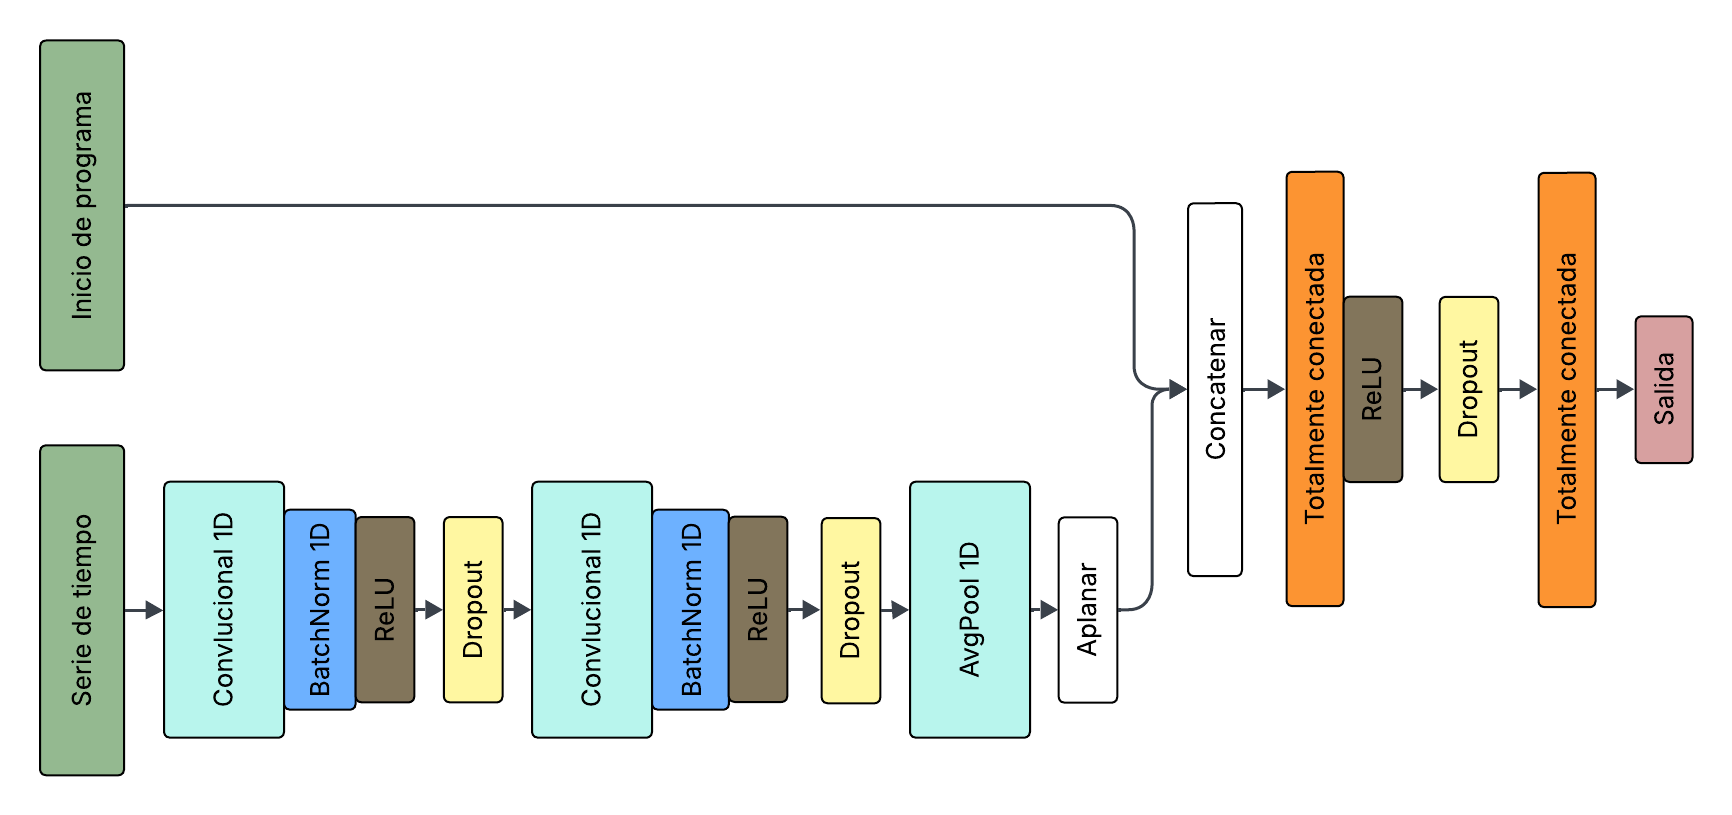
\includegraphics[width=0.8\textwidth]{figs/conv.png}
    \caption{Esquema de la arquitectura de la red convolucional propuesta.}
    \label{fig:conv}
\end{figure}

\subsection{Arquitectura 3: Red Convolucional + LSTM}
Esta última arquitectura combina las otras dos: ahora, el procesamiento de la serie
temporal es llevado a cabo de manera paralela por las capas LSTM de la Arquitectura 1
y las capas convolucionales de la Arquitectura 2. Luego, se combinan ambas salidas y
el inicio de programa para posteriormente producir la predicción final a través de la
red totalmente conectada.
\begin{figure}[h]
    \centering
    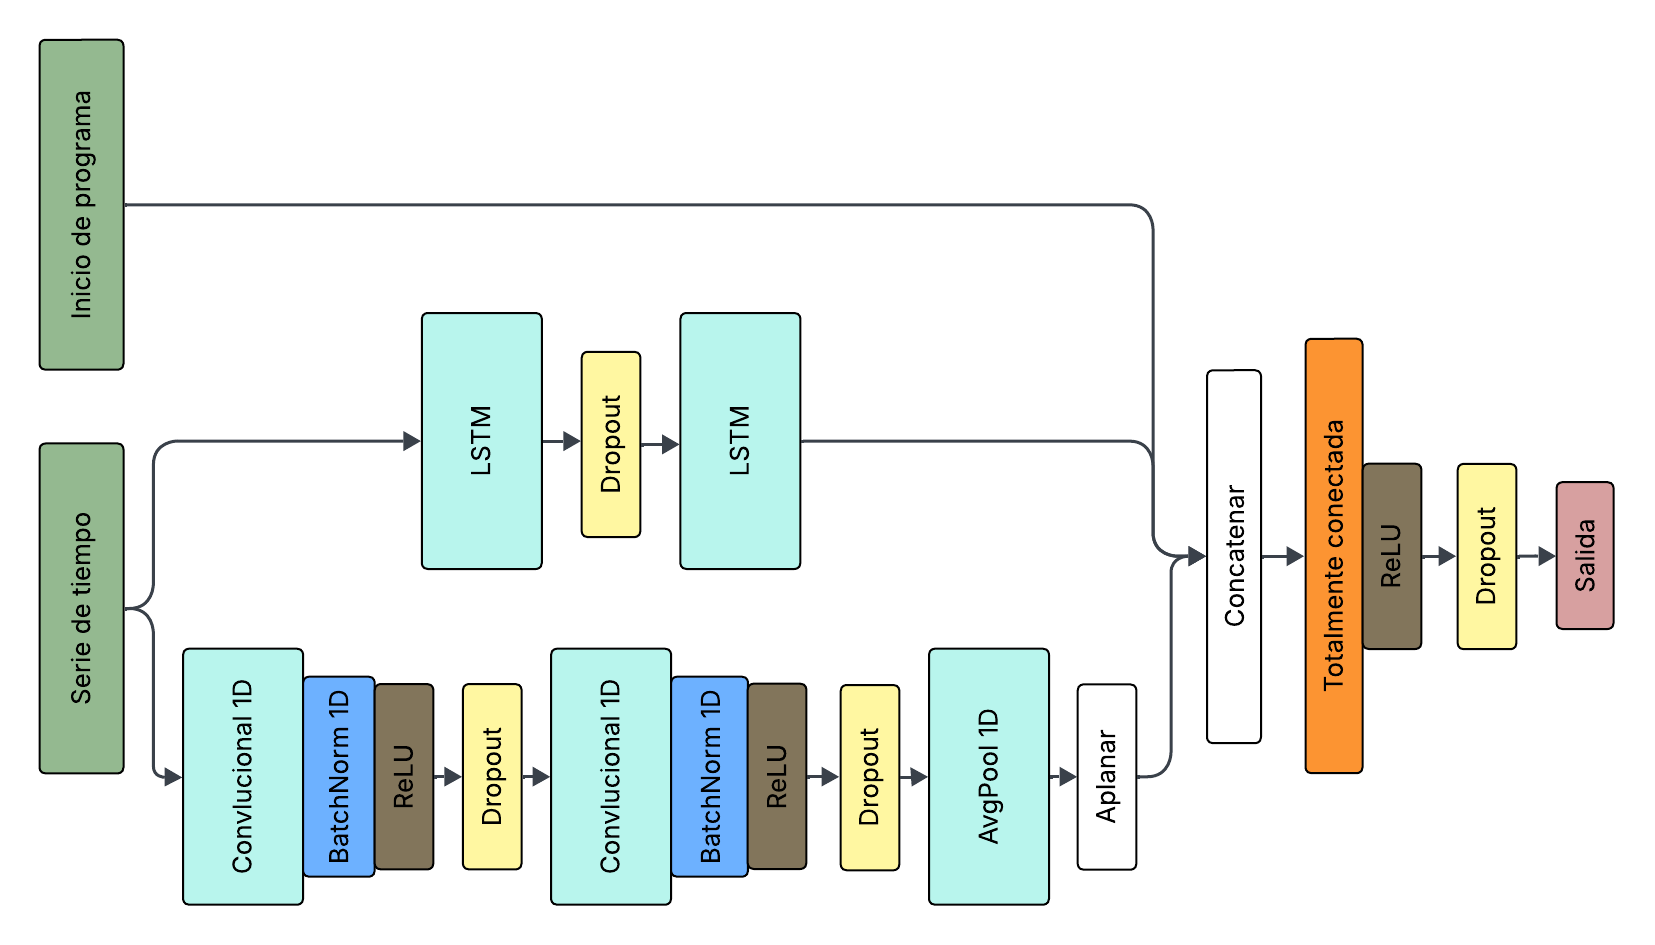
\includegraphics[width=0.8\textwidth]{figs/lstm_conv.png}
    \caption{Esquema de la arquitectura de la red LSTM + convolucional propuesta.}
    \label{fig:lstm_v2_conv}
\end{figure}

\end{document}